\documentclass[10pt,]{article}
\usepackage{lmodern}
\usepackage{amssymb,amsmath}
\usepackage{ifxetex,ifluatex}
\usepackage{fixltx2e} % provides \textsubscript
\ifnum 0\ifxetex 1\fi\ifluatex 1\fi=0 % if pdftex
  \usepackage[T1]{fontenc}
  \usepackage[utf8]{inputenc}
\else % if luatex or xelatex
  \ifxetex
    \usepackage{mathspec}
    \usepackage{xltxtra,xunicode}
  \else
    \usepackage{fontspec}
  \fi
  \defaultfontfeatures{Mapping=tex-text,Scale=MatchLowercase}
  \newcommand{\euro}{€}
\fi
% use upquote if available, for straight quotes in verbatim environments
\IfFileExists{upquote.sty}{\usepackage{upquote}}{}
% use microtype if available
\IfFileExists{microtype.sty}{%
\usepackage{microtype}
\UseMicrotypeSet[protrusion]{basicmath} % disable protrusion for tt fonts
}{}
\usepackage[margin=0.6in]{geometry}
\usepackage{graphicx}
\makeatletter
\def\maxwidth{\ifdim\Gin@nat@width>\linewidth\linewidth\else\Gin@nat@width\fi}
\def\maxheight{\ifdim\Gin@nat@height>\textheight\textheight\else\Gin@nat@height\fi}
\makeatother
% Scale images if necessary, so that they will not overflow the page
% margins by default, and it is still possible to overwrite the defaults
% using explicit options in \includegraphics[width, height, ...]{}
\setkeys{Gin}{width=\maxwidth,height=\maxheight,keepaspectratio}
\ifxetex
  \usepackage[setpagesize=false, % page size defined by xetex
              unicode=false, % unicode breaks when used with xetex
              xetex]{hyperref}
\else
  \usepackage[unicode=true]{hyperref}
\fi
\hypersetup{breaklinks=true,
            bookmarks=true,
            pdfauthor={Ambrosio Q. Tria},
            pdftitle={Motor Trend Project: MPG Analysis},
            colorlinks=true,
            citecolor=blue,
            urlcolor=blue,
            linkcolor=magenta,
            pdfborder={0 0 0}}
\urlstyle{same}  % don't use monospace font for urls
\setlength{\parindent}{0pt}
\setlength{\parskip}{6pt plus 2pt minus 1pt}
\setlength{\emergencystretch}{3em}  % prevent overfull lines
\setcounter{secnumdepth}{0}

%%% Use protect on footnotes to avoid problems with footnotes in titles
\let\rmarkdownfootnote\footnote%
\def\footnote{\protect\rmarkdownfootnote}

%%% Change title format to be more compact
\usepackage{titling}
\setlength{\droptitle}{-2em}
  \title{Motor Trend Project: MPG Analysis}
  \pretitle{\vspace{\droptitle}\centering\huge}
  \posttitle{\par}
  \author{Ambrosio Q. Tria}
  \preauthor{\centering\large\emph}
  \postauthor{\par}
  \date{}
  \predate{}\postdate{}




\begin{document}

\maketitle


{
\hypersetup{linkcolor=black}
\setcounter{tocdepth}{2}
\tableofcontents
}
\begin{center}\rule{0.5\linewidth}{\linethickness}\end{center}

\newpage

\subsection{Preface}\label{preface}

This is the project for the Coursera/ Johns Hopkins Bloomberg School of
Public Health course, Regression Models. It assumes working for Motor
Trend, using the built in data set \texttt{mtcars} to answer
hypothetical questions with analysis and regression modeling. PDF Report
layout comprises of Table of Contents (1 page), Main Body (2 pages), and
Appendix (5 pages).

\hyperdef{}{eo}{\subsection{Executive Summary}\label{eo}}

In order to provide empirical evidence for Motor Trend, this report
presents the analysis of miles per gallon (MPG) on a select collection
of cars. The outcome variable representing MPG will be analyzed against
other variables found in the dataset \texttt{mtcars} using exploratory
data analysis and regression modeling. The analysis will address two
areas of concern:

\begin{enumerate}
\def\labelenumi{\arabic{enumi}.}
\itemsep1pt\parskip0pt\parsep0pt
\item
  Is an automatic or manual transmission better for MPG
\item
  Quantifying the MPG difference between automatic and manual
  transmissions
\end{enumerate}

The analysis and regression modeling shows that manual transmission is
better for MPG when compared to automatic transmission, gven the
interdependence on weight, displacement and number of cylinders.

Supporting figures for the analysis can be found in the
\hyperref[appendix]{Appendix} section of this report. For convenience
throughout the main body of the report, links have been created for
easier navigation to the supporting figures in the appendix.

\hyperdef{}{eda}{\subsection{Exploratory Data Analysis}\label{eda}}

Looking at the structure \{\hyperref[fig1]{figure 1}\} of the dataset
\texttt{mtcars}, we can see that it is comprised of 32 observations on
11 variables, where all variables are numeric. Of the variables listed
and their descriptions \{\hyperref[fig2]{figure 2}\}, the variable
\texttt{am} describes the car's transmission type - boolean values of
{[}1, 0{]}; where 0 is for automatic transmission, and 1 is for manual
transmission per the description \{\hyperref[fig2]{figure 2}\} of
\texttt{am}.

We will copy the original data into a new data frame named
\texttt{mtcars2} where we will assign names to the numerical values of
\texttt{am} in the observations. This will assist with readability in
the plots.

\hyperdef{}{rm}{\subsection{Regression Modeling}\label{rm}}

\subsubsection{SLR modeling}\label{slr-modeling}

Let's take a quick look at fitting a regression model on \texttt{mpg} as
the outcome and the transmission type (\texttt{am}) as the regressor. We
will use a simple linear regression (SLR) model. Its plot
\{\hyperref[fig5]{figure 5}\} shows that manual transmission vehicles
have better \texttt{mpg} than automatic vehicles. This can be
misleading, because as we saw in our exploratory data analysis, there
are other variables in the dataset that can potentially impact
\texttt{mpg}, which is not accounted for in this simple plot.

Let's try to validate this by taking its residual to confirm if the SLR
model is a good fit. We see that its plot does not show the scatter we
expect from a residual. In fact, it is exactly as the SLR plot. It is
unquestionable that the SLR model is not a good fit for \texttt{mpg} vs
Transmission Type. And as expected, it does not account for data between
the two Transmission Type points - it simply cannot, given only 2 values
for the x axis. You can see these results in \{\hyperref[fig5]{figure
5}\}.

Finally, let's confirm if other variables in the data set impact
\texttt{mpg}. Taking a look at the SLR of \texttt{mpg} versus horsepower
(\texttt{hp}), you can see a linear decrease for \texttt{mpg} as
horsepower increases for both automatic and manual transmissions,
opposite than what we saw in the SLR for \texttt{mpg} versus
Transmission Type. Its residual plot is more reasonable than what we saw
before; however, there seems to be a secondary linear pattern showing
for both automatic and manual transmission, suggesting a relationship
with one or more other variables in the dataset. You can see this in
\{\hyperref[fig6]{figure 6}\}.

From these results, we've confirmed that other variables in the data set
do have an impact on \texttt{mpg}, as well as on each other. Therefore,
we will need to apply a different regression model to the data set.
Before we do, we will assess which variables to include and which to
exclude.

\subsubsection{Multivariate regression
modeling}\label{multivariate-regression-modeling}

We will use a multivariate linear regression model on the dataset. The
multivariate regression summary of \texttt{mpg} vs all the other
variables \{\hyperref[fig7]{figure 7}\} gives us the coefficients to
interpret the impact of each variable in the dataset on \texttt{mpg}, as
they are influenced by every other variable held at that particular
time.

From this multivariate model, and a listing of the different
correlations with mpg, we will select a subset of variables that have
the most impact on \texttt{mpg}, and create a focused multivariate
model. So, from the summary \{\hyperref[fig7]{figure 7}\}, the variable
with the most significance is \texttt{wt} (weight), although its
significance is not a strong significance as shown by its p-value. The
coefficients tell us that for every unit increase of \texttt{wt}, mpg
decreases by -3.7. The transmission type \texttt{am} is the next largest
change in \texttt{mpg}, in the positive direction, with a coefficient of
2.5. Interestingly enough, the \texttt{am} p-value is not great.

On the other hand, the table of \texttt{mpg} correlations with each
variable \{\hyperref[fig8]{figure 8}\} shows that the strongest
correlations with \texttt{mpg} are with weight (\texttt{wt}),
displacement (\texttt{disp}), and cylinder (\texttt{cyl}).

Based on coefficient significance and correlation strength, we will
create a multivariate model of \texttt{mpg} vs \texttt{am} + \texttt{wt}
+ \texttt{disp} + \texttt{cyl} as the model to answer our questions.
Let's confirm this final model.

We take the first SLR model \{\hyperref[fig5]{figure 5}\} that we
created and use that to build subsequent updated models and test them
via ANOVA. The result of our final model choice of
\texttt{mpg\ \textasciitilde{}\ am\ +\ wt\ +\ disp\ +\ cyl}
\{\hyperref[anova1]{figure 11}\} is a good fit, where the p-values of
\texttt{am\ +\ wt} and \texttt{am\ +\ wt\ +\ disp\ +\ cyl} are
significant. To verify that other variables are not impacting on our
selected model, we sample two other variables and fit models adding
\texttt{qsec} \{\hyperref[anova2]{figure 12}\}and then adding
\texttt{hp} \{\hyperref[anova3]{figure 13}\} (remember, we looked at
\texttt{hp} in an SLR). The ANOVA models show that these additions are
not significant and we can leave out \texttt{qsec} and \texttt{hp}.

We have our final regression summary \{\hyperref[fig9]{figure 9}\} and
visualization plot \{\hyperref[fig10]{figure 10}\} of our selected
model.

\hyperdef{}{conclusion}{\subsection{Conclusion}\label{conclusion}}

We should be clear that the dataset \texttt{mtcars} is very limited with
number of observations and randomness, and is aged. It is a data source
from 1974.

So, from the multivariate regression model we selected, we can see that
transmission type is very dependent on the other variables, the other
vehicular attributes when analyzing miles per gallon (\texttt{mpg}).
Weight (\texttt{wt}) has a significant and strong relationship with
transmission type (\texttt{am}). Both \texttt{am} and \texttt{wt} are
influenced by displacement (\texttt{disp}) and number of cylinders
(\texttt{cyl}). Looking at the plot of these relationships over
transmission types \{\hyperref[fig10]{figure 10}\}, we can see that
manual transmissions have an initial advantage over automatic
transmissions for \texttt{mpg}, and that the influencial relationships
with the change in other vehicular attributes show an increase in
\texttt{mpg} for manual transmissions. Automatic transmissions slightly
affect \texttt{mpg} positively as the other attributes are changed.
Overall, manual transmissions is a better design for \texttt{mpg}.
Improvements in the other vehicular attributes do have positive
influence for \texttt{mpg} in both transmission types.

Note: This report was authored in R Markdown and compiled to pdf using
pdflatex (via knitr)\footnote{To view the raw source and for
  reproducibility, please visit my Github
  \href{https://github.com/AmbroseT/RegressionModels}{repository}}.
Figure 3 and figure 4 were omitted due to space constraints.

\newpage

\hyperdef{}{appendix}{\section{Appendix}\label{appendix}}

All supporting figures can be found in this appendix. For convenience,
links have been created for easier navigation back to the main body of
the report. Note that captions for the figures have been left out
because of the linked figure titles.

\hyperdef{}{fig1}{\subsection{Figure 1: Structure of the dataset
MTCARS}\label{fig1}}

\begin{verbatim}
## 'data.frame':    32 obs. of  11 variables:
##  $ mpg : num  21 21 22.8 21.4 18.7 18.1 14.3 24.4 22.8 19.2 ...
##  $ cyl : num  6 6 4 6 8 6 8 4 4 6 ...
##  $ disp: num  160 160 108 258 360 ...
##  $ hp  : num  110 110 93 110 175 105 245 62 95 123 ...
##  $ drat: num  3.9 3.9 3.85 3.08 3.15 2.76 3.21 3.69 3.92 3.92 ...
##  $ wt  : num  2.62 2.88 2.32 3.21 3.44 ...
##  $ qsec: num  16.5 17 18.6 19.4 17 ...
##  $ vs  : num  0 0 1 1 0 1 0 1 1 1 ...
##  $ am  : num  1 1 1 0 0 0 0 0 0 0 ...
##  $ gear: num  4 4 4 3 3 3 3 4 4 4 ...
##  $ carb: num  4 4 1 1 2 1 4 2 2 4 ...
\end{verbatim}

\hyperref[eo]{Executive Summary} \textbar{} \hyperref[eda]{Exploratory
Data Analysis} \textbar{} \hyperref[rm]{Regression Modeling} \textbar{}
\hyperref[conclusion]{Conclusion}

\hyperdef{}{fig2}{\subsection{Figure 2: Dataset Variable
Description}\label{fig2}}

\begin{verbatim}
##    VARIABLE                              DESCRIPTION
## 1       mpg                        Miles/(US) gallon
## 2       cyl                      Number of cylinders
## 3      disp                    Displacement (cu.in.)
## 4        hp                         Gross horsepower
## 5      drat                          Rear axle ratio
## 6        wt                         Weight (lb/1000)
## 7      qsec                            1/4 mile time
## 8        vs                                      V/S
## 9        am Transmission (0 = automatic, 1 = manual)
## 10     gear                  Number of forward gears
## 11     carb                    Number of carburetors
\end{verbatim}

\hyperref[eo]{Executive Summary} \textbar{} \hyperref[eda]{Exploratory
Data Analysis} \textbar{} \hyperref[rm]{Regression Modeling} \textbar{}
\hyperref[conclusion]{Conclusion}

\hyperdef{}{fig5}{\subsection{Figure 5: SLR of MPG vs Transmission Type,
and its Residual Plot}\label{fig5}}

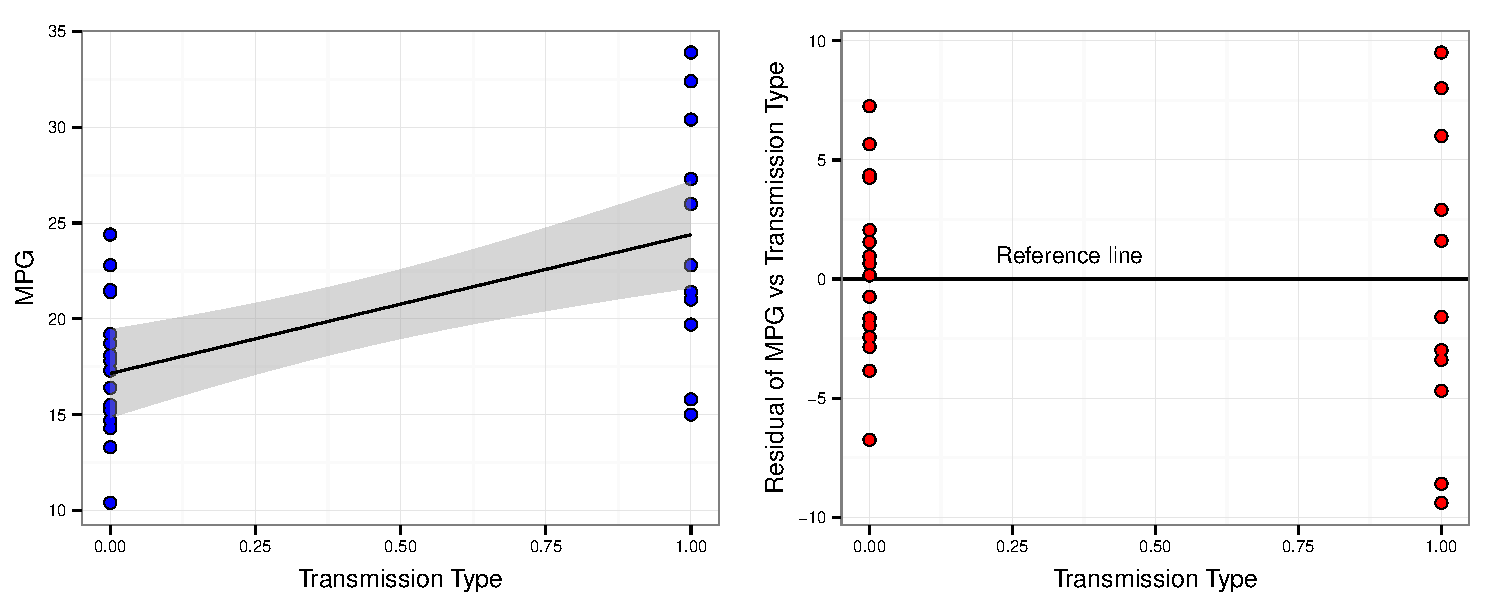
\includegraphics{RegressionModelsProj_3_files/figure-latex/unnamed-chunk-10-1.pdf}

\hyperref[eo]{Executive Summary} \textbar{} \hyperref[eda]{Exploratory
Data Analysis} \textbar{} \hyperref[rm]{Regression Modeling} \textbar{}
\hyperref[conclusion]{Conclusion}

\hyperdef{}{fig6}{\subsection{Figure 6: SLR of MPG vs Horsepower for
Transmission Types, and its Residual Plot}\label{fig6}}

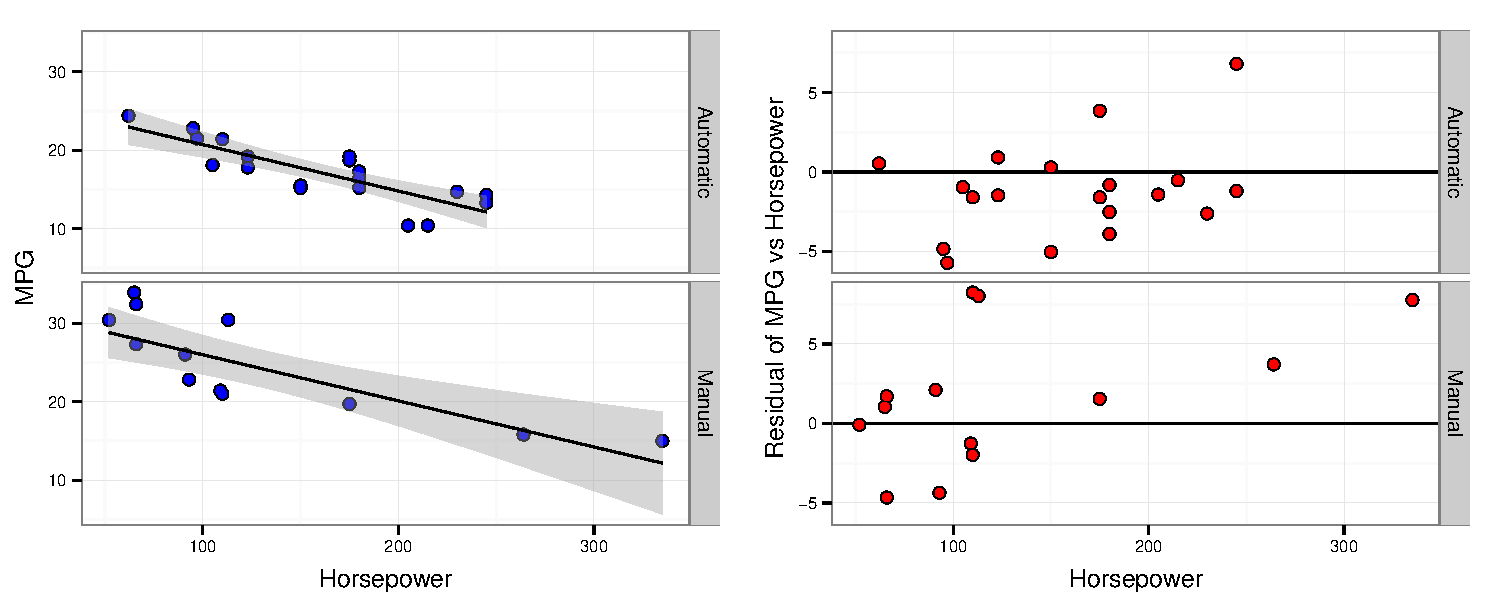
\includegraphics{RegressionModelsProj_3_files/figure-latex/unnamed-chunk-11-1.pdf}

\hyperref[eo]{Executive Summary} \textbar{} \hyperref[eda]{Exploratory
Data Analysis} \textbar{} \hyperref[rm]{Regression Modeling} \textbar{}
\hyperref[conclusion]{Conclusion}

\hyperdef{}{fig7}{\subsection{Figure 7: Regression Summary of MPG vs all
other variables}\label{fig7}}

\begin{verbatim}
## 
## Call:
## lm(formula = mpg ~ ., data = mtcars)
## 
## Residuals:
##     Min      1Q  Median      3Q     Max 
## -3.4506 -1.6044 -0.1196  1.2193  4.6271 
## 
## Coefficients:
##             Estimate Std. Error t value Pr(>|t|)  
## (Intercept) 12.30337   18.71788   0.657   0.5181  
## cyl         -0.11144    1.04502  -0.107   0.9161  
## disp         0.01334    0.01786   0.747   0.4635  
## hp          -0.02148    0.02177  -0.987   0.3350  
## drat         0.78711    1.63537   0.481   0.6353  
## wt          -3.71530    1.89441  -1.961   0.0633 .
## qsec         0.82104    0.73084   1.123   0.2739  
## vs           0.31776    2.10451   0.151   0.8814  
## am           2.52023    2.05665   1.225   0.2340  
## gear         0.65541    1.49326   0.439   0.6652  
## carb        -0.19942    0.82875  -0.241   0.8122  
## ---
## Signif. codes:  0 '***' 0.001 '**' 0.01 '*' 0.05 '.' 0.1 ' ' 1
## 
## Residual standard error: 2.65 on 21 degrees of freedom
## Multiple R-squared:  0.869,  Adjusted R-squared:  0.8066 
## F-statistic: 13.93 on 10 and 21 DF,  p-value: 3.793e-07
\end{verbatim}

\hyperref[eo]{Executive Summary} \textbar{} \hyperref[eda]{Exploratory
Data Analysis} \textbar{} \hyperref[rm]{Regression Modeling} \textbar{}
\hyperref[conclusion]{Conclusion}

\hyperdef{}{fig8}{\subsection{Figure 8: Correlations Table of MPG and
Each Variable in the dataset}\label{fig8}}

\begin{tabular}{rrrr}
  \hline
 & 1st Variable & 2nd Variable & Correlation \\ 
  \hline
1 & mpg & cyl & -0.85 \\ 
  2 & mpg & disp & -0.85 \\ 
  3 & mpg & hp & -0.78 \\ 
  4 & mpg & drat & 0.68 \\ 
  5 & mpg & wt & -0.87 \\ 
  6 & mpg & qsec & 0.42 \\ 
  7 & mpg & vs & 0.66 \\ 
  8 & mpg & am & 0.6 \\ 
  9 & mpg & gear & 0.48 \\ 
  10 & mpg & carb & -0.55 \\ 
   \hline
\end{tabular}

\hyperref[eo]{Executive Summary} \textbar{} \hyperref[eda]{Exploratory
Data Analysis} \textbar{} \hyperref[rm]{Regression Modeling} \textbar{}
\hyperref[conclusion]{Conclusion}

\hyperdef{}{fig9}{\subsection{Figure 9: Regression Summary of MPG vs
Select Variables}\label{fig9}}

\begin{verbatim}
## 
## Call:
## lm(formula = mpg ~ am + wt + disp + cyl, data = mtcars)
## 
## Residuals:
##    Min     1Q Median     3Q    Max 
## -4.318 -1.362 -0.479  1.354  6.059 
## 
## Coefficients:
##              Estimate Std. Error t value Pr(>|t|)    
## (Intercept) 40.898313   3.601540  11.356 8.68e-12 ***
## am           0.129066   1.321512   0.098  0.92292    
## wt          -3.583425   1.186504  -3.020  0.00547 ** 
## disp         0.007404   0.012081   0.613  0.54509    
## cyl         -1.784173   0.618192  -2.886  0.00758 ** 
## ---
## Signif. codes:  0 '***' 0.001 '**' 0.01 '*' 0.05 '.' 0.1 ' ' 1
## 
## Residual standard error: 2.642 on 27 degrees of freedom
## Multiple R-squared:  0.8327, Adjusted R-squared:  0.8079 
## F-statistic: 33.59 on 4 and 27 DF,  p-value: 4.038e-10
\end{verbatim}

\hyperref[eo]{Executive Summary} \textbar{} \hyperref[eda]{Exploratory
Data Analysis} \textbar{} \hyperref[rm]{Regression Modeling} \textbar{}
\hyperref[conclusion]{Conclusion}

\hyperdef{}{fig10}{\subsection{Figure 10: Visualization of Regression
Summary of MPG}\label{fig10}}

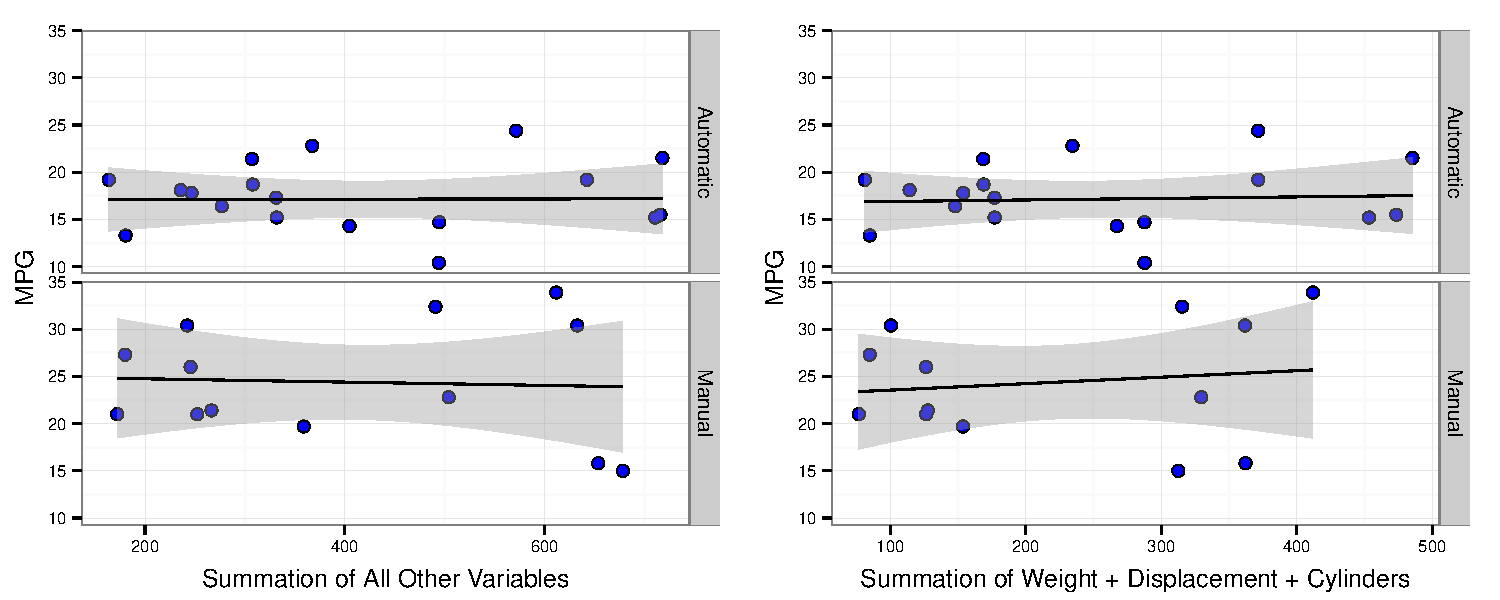
\includegraphics{RegressionModelsProj_3_files/figure-latex/unnamed-chunk-15-1.pdf}

\hyperref[eo]{Executive Summary} \textbar{} \hyperref[eda]{Exploratory
Data Analysis} \textbar{} \hyperref[rm]{Regression Modeling} \textbar{}
\hyperref[conclusion]{Conclusion}

\hyperdef{}{anova1}{\subsection{Figure 11: ANOVA Table 1, Our Selected
Model Test}\label{anova1}}

\begin{verbatim}
## Analysis of Variance Table
## 
## Model 1: mpg ~ am
## Model 2: mpg ~ am + wt
## Model 3: mpg ~ am + wt + disp + cyl
##   Res.Df    RSS Df Sum of Sq       F    Pr(>F)    
## 1     30 720.90                                   
## 2     29 278.32  1    442.58 63.4179 1.469e-08 ***
## 3     27 188.43  2     89.89  6.4406  0.005165 ** 
## ---
## Signif. codes:  0 '***' 0.001 '**' 0.01 '*' 0.05 '.' 0.1 ' ' 1
\end{verbatim}

\hyperref[eo]{Executive Summary} \textbar{} \hyperref[eda]{Exploratory
Data Analysis} \textbar{} \hyperref[rm]{Regression Modeling} \textbar{}
\hyperref[conclusion]{Conclusion}

\hyperdef{}{anova2}{\subsection{Figure 12: ANOVA Table 2, Adding
QSEC}\label{anova2}}

\begin{verbatim}
## Analysis of Variance Table
## 
## Model 1: mpg ~ am
## Model 2: mpg ~ am + wt
## Model 3: mpg ~ am + wt + disp + cyl
## Model 4: mpg ~ wt + disp + cyl + qsec
##   Res.Df    RSS Df Sum of Sq       F    Pr(>F)    
## 1     30 720.90                                   
## 2     29 278.32  1    442.58 63.4179 1.469e-08 ***
## 3     27 188.43  2     89.89  6.4406  0.005165 ** 
## 4     27 175.67  0     12.76                      
## ---
## Signif. codes:  0 '***' 0.001 '**' 0.01 '*' 0.05 '.' 0.1 ' ' 1
\end{verbatim}

\hyperref[eo]{Executive Summary} \textbar{} \hyperref[eda]{Exploratory
Data Analysis} \textbar{} \hyperref[rm]{Regression Modeling} \textbar{}
\hyperref[conclusion]{Conclusion}

\hyperdef{}{anova3}{\subsection{Figure 13: ANOVA Table 3, Adding
HP}\label{anova3}}

\begin{verbatim}
## Analysis of Variance Table
## 
## Model 1: mpg ~ am
## Model 2: mpg ~ am + wt
## Model 3: mpg ~ am + wt + disp + cyl
## Model 4: mpg ~ wt + disp + cyl + qsec
## Model 5: mpg ~ wt + disp + cyl + hp
##   Res.Df    RSS Df Sum of Sq       F    Pr(>F)    
## 1     30 720.90                                   
## 2     29 278.32  1    442.58 63.4179 1.469e-08 ***
## 3     27 188.43  2     89.89  6.4406  0.005165 ** 
## 4     27 175.67  0     12.76                      
## 5     27 170.44  0      5.22                      
## ---
## Signif. codes:  0 '***' 0.001 '**' 0.01 '*' 0.05 '.' 0.1 ' ' 1
\end{verbatim}

\hyperref[eo]{Executive Summary} \textbar{} \hyperref[eda]{Exploratory
Data Analysis} \textbar{} \hyperref[rm]{Regression Modeling} \textbar{}
\hyperref[conclusion]{Conclusion}

\end{document}
